\newcommand{\QthreeCost}{13,207,966.05}
\newcommand{\QthreeCostWan}{1320.7966}
\newcommand{\QthreeEmergency}{41,443.14}
\newcommand{\QthreeEmergencyCost}{228,716.57}
\newcommand{\QthreeOriginal}{20,880,166.69}
\newcommand{\QthreeContract}{20,680,999.57}
\newcommand{\QthreeCharge}{6,601,919.54}
\newcommand{\QthreeDischarge}{5,350,750.77}
\newcommand{\QthreeEnd}{2,448.95}
\newcommand{\QthreeUnusedPV}{1,149,260.85}
\newcommand{\QthreeUnusedGrid}{382,823.59}
\newcommand{\QthreeInformationSaving}{67,227.15}
\newcommand{\QthreeInformationRate}{0.5064}
\newcommand{\QthreeEvents}{316}
\newcommand{\QthreeEmergencyDays}{171}
\newcommand{\QthreeEmergencyIntervals}{696}

\section{问题三：基于滚动预报的购电调整与储能控制}
\label{sec:q3}

\subsection{问题分析}

问题三在问题二基础上增加0:00、6:00、12:00和18:00发布的光伏预报，并允许对待交付的购电计划付费调整。若一次更新直接修改其后的全部计划，则6:00预报会对12:00以后的电量提前形成交易，而这些时段还会获得更新信息。本文采用“全日规划、六小时更新”的滚动机制：每次规划至当日24:00，但日内只确认至下一发布时间的购电量，其余结果用于估计当前储能对后续时段的作用。

储能采用递减价值DP控制。每个发布时间根据当时可用的预报和历史误差重建剩余日价值函数，并执行随后6小时。实际储电量连续传递至下一发布时间和次日。

图\ref{fig:q3-workflow}概括光伏预报处理、策略分段更新、储能控制和费用核验流程。

\begin{figure}[H]
    \centering
    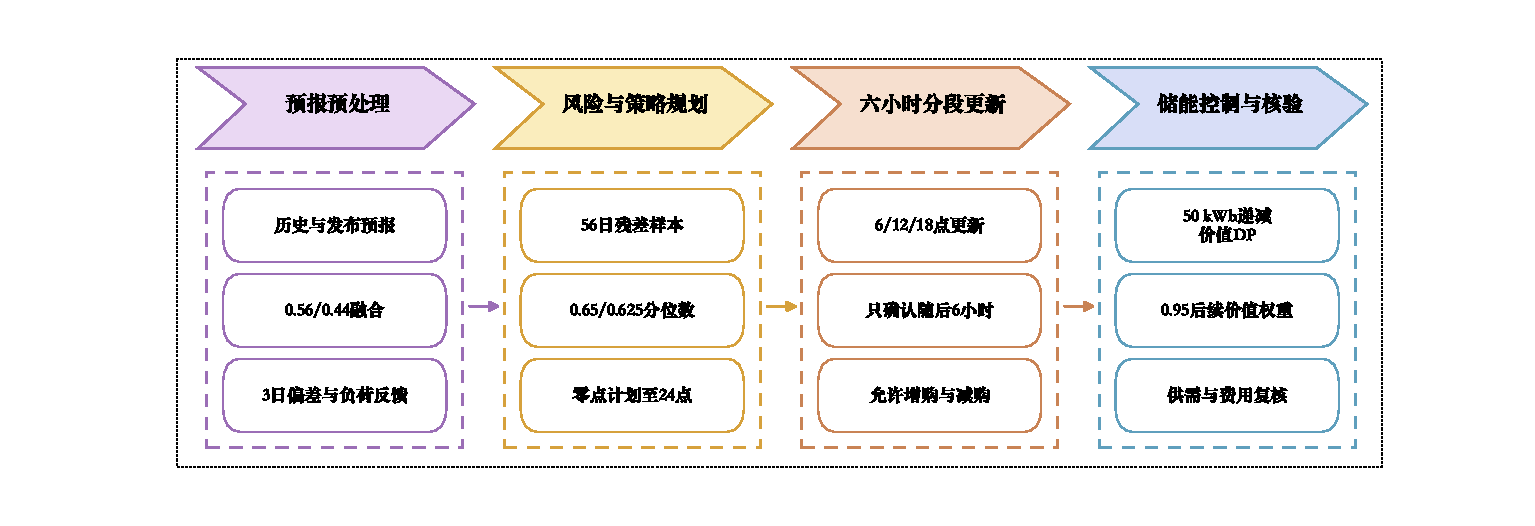
\includegraphics[width=\textwidth,trim=28mm 8mm 24mm 8mm,clip]{figures/q3/flowchart3.pdf}
    \caption{问题三流程图}
    \label{fig:q3-workflow}
\end{figure}

\subsection{预报处理与信息范围}

\subsubsection{发布时间与交付区间}

沿用日期$k$和区间$t=0,\ldots,T-1$，其中$T=144$、$\Delta t=1/6\,\mathrm h$。令$r=0,1,2,3$表示四个发布时间，$s_r=36r$为对应区间编号，并定义
\begin{equation}
    \mathcal I_r=\{s_r,\ldots,\min(s_r+35,T-1)\},\qquad
    \mathcal H_r=\{s_r,\ldots,T-1\}.
    \label{eq:q3-windows}
\end{equation}
$\mathcal I_r$是本次确认的交付窗口，$\mathcal H_r$是规划视野。0:00形成全天计划；6:00、12:00和18:00分别只调整6:00--12:00、12:00--18:00和18:00--24:00的计划。因此每个交付区间除零点基础交易外，至多发生一次日内调整。

\subsubsection{光伏预报融合与安全余量}

附件3的整点功率预报先截为非负，在相邻整点间线性插值，再按梯形积分换算为十分钟电量。发布时刻的插值起点取此前最后一个完整实测区间。记发布预报和历史光伏预测为$\widehat V_{k,r,\ell}^{\rm pub}$与$\widehat V_{k,r,\ell}^{\rm hist}$，融合结果为
\begin{equation}
 \widehat V_{k,r,\ell}
 =\left[0.56\widehat V_{k,r,\ell}^{\rm pub}
 +0.44\widehat V_{k,r,\ell}^{\rm hist}+\delta_{k,r,\ell}^{\rm PV}\right]_+,
 \label{eq:q3-pv-correction}
\end{equation}
其中$\delta_{k,r,\ell}^{\rm PV}$取最近至多3个完整日同一发布时间和提前区间的平均预测误差。

负载预测在昨日同刻、上周同刻和Ridge之间按最近14个完整日的误差滚动选择，并进行近3日偏差修正。日内预测再利用最近2小时已经发生的负载误差进行反馈，初始权重为0.5，影响随预测距离衰减。

对每个发布时间和相对小时$h(\ell)=\lfloor\ell/6\rfloor$，汇集此前最多56个完整日的净负载残差，形成集合$\mathcal R_{k,r,h(\ell)}$。安全余量取
\begin{equation}
 m_{k,r,\ell}=\max\left\{0,Q_{\alpha_r}\!\left(\mathcal R_{k,r,h(\ell)}\right)\right\},
 \qquad \alpha_0=0.65,\quad\alpha_1=\alpha_2=\alpha_3=0.625.
 \label{eq:q3-margin}
\end{equation}
不同发布时间下的预测误差和调整费用不同，两个分位数根据历史数据复算确定，在评估期内保持不变。

\textbf{参数确定。}参数比较以总费用为主要指标，同时记录紧急购电量和未利用电量。将零点及日内分位数均提高至0.8而保持其余设置不变时，总费用由1320.7966万元增至1351.9329万元，紧急购电量由4.1443万\,kWh降至1.2962万\,kWh，未利用电量由153.2084万\,kWh增至211.6474万\,kWh。较高分位数以31.1363万元额外费用换取2.8481万\,kWh紧急购电量下降，因此主方案采用0.65和0.625。

融合权重、56日残差窗口、2400/6000\,kWh参考量和0.95后续价值权重在同一历史复算中固定，分别控制预报融合、残差样本量、日末留电和后续电量价值。

图\ref{fig:q3-forecast}给出3月20日各发布时间后六小时内送入规划模型的光伏预报。竖虚线表示信息更新点。

\begin{figure}[H]
    \centering
    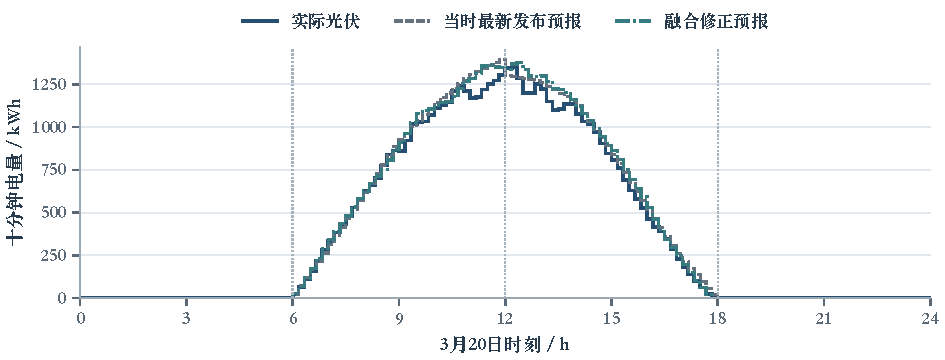
\includegraphics[width=\textwidth]{figures/q3/q3_forecast.pdf}
    \caption{指定日光伏实测、发布预报与融合修正结果}
    \label{fig:q3-forecast}
\end{figure}

\subsection{滚动购电模型}

\subsubsection{基础计划与调整费用}

令$q_{kt}^{0}$为0:00确定的基础购电量，$q_{kt}^{\rm f}$为最终确认量，并定义
\begin{equation}
 a_{kt}=(q_{kt}^{\rm f}-q_{kt}^{0})_+,
 \qquad b_{kt}=(q_{kt}^{0}-q_{kt}^{\rm f})_+.
 \label{eq:q3-adjustment}
\end{equation}
增购部分按$1.5p_t$计费。减购时退回原购电费，同时对取消部分支付$0.5p_t$违约费。每个区间的实际费用为
\begin{equation}
 C_{kt}=p_tq_{kt}^{0}+1.5p_ta_{kt}-0.5p_tb_{kt}+5p_tu_{kt}
 =p_tq_{kt}^{\rm f}+0.5p_t\lvert q_{kt}^{\rm f}-q_{kt}^{0}\rvert+5p_tu_{kt}.
 \label{eq:q3-actual-cost}
\end{equation}
例如，原计划100\,kWh、最终确认80\,kWh且$p_t=1$时，该区间普通购电费用为90元。

\subsubsection{零点计划与日内滚动优化}

0:00根据融合预报和安全余量求解全天计划，初始储电量取实际值，计划日末储电量固定为2400\,kWh。6:00、12:00和18:00重新计算$\mathcal H_r$内的购电和储能安排，但只将$\mathcal I_r$内的结果写入策略。

对$t\in\mathcal I_r$，记本次规划相对零点策略的增购量和减购量为$a_{kt}^{(r)}$、$b_{kt}^{(r)}$，日末储电量低于6000\,kWh的部分为$\xi_{kr}$。日内目标为
\begin{equation}
\begin{aligned}
 \min\quad
 &\sum_{t\in\mathcal I_r}\left(1.5p_ta_{kt}^{(r)}-0.5p_tb_{kt}^{(r)}+5p_t\bar u_{kt}\right)\\
 &+\sum_{t\in\mathcal H_r\setminus\mathcal I_r}
 \left(p_t\widetilde q_{kt}^{(r)}+5p_t\bar u_{kt}\right)
 +\lambda_{kr}\xi_{kr},
\end{aligned}
\label{eq:q3-rolling-objective}
\end{equation}
其中$\lambda_{kr}=1.5\min_{t\in\mathcal H_r}p_t/\eta_c$。规划轨迹满足供需平衡、储电量递推、容量和功率约束，并有
\begin{equation}
 \bar E_{k,s_r}=E_{k,s_r},\qquad
 \bar E_{k,T}+\xi_{kr}\ge6000.
 \label{eq:q3-physical}
\end{equation}
未来窗口内尚未确认的购电量只参与本次规划，下一发布时间重新计算。

\subsubsection{递减价值DP控制}

设$\varepsilon_t$为相同发布时间和小时内的历史净负载残差。给定已确认策略，剩余日储能费用函数满足
\begin{equation}
 \mathcal V_{k,t}^{(r)}(E)=
 \mathbb E_{\varepsilon_t}\!\left[
 \min_{E'}\left\{5p_tu_t(E,E',\varepsilon_t)
 +0.95\mathcal V_{k,t+1}^{(r)}(E')\right\}\right].
 \label{eq:q3-value-dp}
\end{equation}
每个发布时间和相对小时内的历史残差按相同权重组成历史残差分布，不同时段的残差在递推中独立取样，DP状态只保留储电量。每次获得新预报后重新计算残差分布和价值函数，使控制结果随最新信息更新。
日末补电费用估计为
\begin{equation}
 \mathcal V_{k,T}^{(r)}(E)=\lambda_{kr}(6000-E)_+.
 \label{eq:q3-terminal-value}
\end{equation}
储电量按50\,kWh划分为193个网格点，实际储电量保持连续，网格间采用线性插值。四次DP分别覆盖144、108、72和36个区间，各执行前36个区间后重建。

\subsection{求解结果}

\subsubsection{全年费用与储能运行}

评估期为2025年2月1日至12月31日，共334天。零点计划量、最终策略量和紧急购电量分别为2088.0167万、2068.1000万和4.1443万\,kWh。原策略费为1,274.6717万元，增购费39.4426万元，减购违约费16.1894万元，退回原策略费用32.3788万元，紧急购电费22.8717万元，总费用为\QthreeCost{}元，即\QthreeCostWan{}万元。

累计充电\QthreeCharge\,kWh、放电\QthreeDischarge\,kWh，均按交流侧计量；年末实际储电量为\QthreeEnd\,kWh。紧急购电发生在\QthreeEmergencyDays{}天的\QthreeEmergencyIntervals{}个十分钟区间，按同日连续区间合并为\QthreeEvents{}次事件。

\subsubsection{指定日期结果}

表\ref{tab:q3-purchase}给出四个指定日期的零点计划与最终确认量，表\ref{tab:q3-storage}汇总实际充放电和日初末储电量。

\begin{table}[H]
    \centering\small
    \caption{指定日期原计划与最终普通购电量（电量单位：kWh）}
    \label{tab:q3-purchase}
    \renewcommand{\arraystretch}{1.18}
    \begingroup
\setlength{\tabcolsep}{2pt}
\begin{tabularx}{\textwidth}{@{}>{\columncolor{white}[0pt][\tabcolsep]}lX *{3}{rrX}r>{\columncolor{white}[\tabcolsep][0pt]}r@{}}
\toprule
\rowcolor{paperpale} 时间段 &  & \multicolumn{2}{c}{\mbox{3月20日}} &  & \multicolumn{2}{c}{\mbox{6月21日}} &  & \multicolumn{2}{c}{\mbox{9月23日}} &  & \multicolumn{2}{>{\columncolor{white}[\tabcolsep][0pt]}c@{}}{\mbox{12月21日}} \\
\rowcolor{paperpale} &  & 原计划 & 最终量 &  & 原计划 & 最终量 &  & 原计划 & 最终量 &  & 原计划 & 最终量  \\
\midrule
10:00--10:10 &  & 0.00 & 0.00 &  & 0.00 & 0.00 &  & 0.00 & 0.00 &  & 0.00 & 0.00  \\
\rowcolor{paperstripe} 12:00--12:10 &  & 507.99 & 507.99 &  & 0.00 & 0.00 &  & 432.96 & 402.61 &  & 965.58 & 900.26  \\
14:00--14:10 &  & 0.00 & 0.00 &  & 0.00 & 0.00 &  & 0.00 & 0.00 &  & 0.00 & 0.00  \\
\rowcolor{paperstripe} 16:00--16:10 &  & 565.06 & 471.42 &  & 194.08 & 151.23 &  & 542.37 & 542.37 &  & 810.25 & 825.26  \\
18:00--18:10 &  & 710.96 & 710.96 &  & 0.00 & 0.00 &  & 788.93 & 777.54 &  & 692.42 & 685.03  \\
\rowcolor{paperstripe} 20:00--20:10 &  & 0.00 & 0.00 &  & 0.00 & 0.00 &  & 0.00 & 0.00 &  & 0.00 & 0.00  \\
全天电量 &  & 68,629.91 & 66,728.81 &  & 34,088.88 & 33,892.35 &  & 70,210.20 & 68,480.54 &  & 95,973.04 & 95,514.31  \\
\rowcolor{paperstripe} 普通购电费/元 &  & 41,911.29 & 42,276.67 &  & 19,406.33 & 19,384.56 &  & 43,668.60 & 43,244.97 &  & 61,414.04 & 62,051.99  \\
\bottomrule
\end{tabularx}


\endgroup

\end{table}

\begin{table}[H]
    \centering\small
    \caption{指定日期各四小时时段的实际充放电量与首末储电量（kWh）}
    \label{tab:q3-storage}
    \renewcommand{\arraystretch}{1.18}
    \begingroup
\setlength{\tabcolsep}{2pt}
\begin{tabularx}{\textwidth}{@{}>{\columncolor{white}[0pt][\tabcolsep]}lX *{3}{rrX}r>{\columncolor{white}[\tabcolsep][0pt]}r@{}}
\toprule
\rowcolor{paperpale} 时间段 &  & \multicolumn{2}{c}{\mbox{3月20日}} &  & \multicolumn{2}{c}{\mbox{6月21日}} &  & \multicolumn{2}{c}{\mbox{9月23日}} &  & \multicolumn{2}{>{\columncolor{white}[\tabcolsep][0pt]}c@{}}{\mbox{12月21日}} \\
\rowcolor{paperpale} &  & 充电 & 放电 &  & 充电 & 放电 &  & 充电 & 放电 &  & 充电 & 放电  \\
\midrule
00:00--04:00 &  & 7,300.40 & 76.23 &  & 374.97 & 402.69 &  & 7,925.24 & 20.92 &  & 7,653.53 & 264.36  \\
\rowcolor{paperstripe} 04:00--08:00 &  & 1,692.23 & 5,668.18 &  & 1,183.25 & 1,759.53 &  & 1,163.69 & 6,545.23 &  & 2,811.36 & 1,726.88  \\
08:00--12:00 &  & 4,920.46 & 2,777.38 &  & 10,187.95 & 0.00 &  & 5,091.10 & 1,896.62 &  & 5,181.38 & 7,718.68  \\
\rowcolor{paperstripe} 12:00--16:00 &  & 5,083.74 & 482.49 &  & 0.00 & 0.00 &  & 5,701.49 & 541.87 &  & 7,963.47 & 2,018.59  \\
16:00--20:00 &  & 285.30 & 5,257.98 &  & 109.30 & 5,912.38 &  & 230.95 & 5,682.33 &  & 23.91 & 5,841.92  \\
\rowcolor{paperstripe} 20:00--24:00 &  & 1,754.17 & 2,901.87 &  & 2,111.57 & 2,621.68 &  & 1,966.72 & 2,997.11 &  & 1,765.67 & 2,832.89  \\
0:00储电量 &  & \multicolumn{2}{r}{2,919.07} &  & \multicolumn{2}{r}{2,630.91} &  & \multicolumn{2}{r}{2,768.35} &  & \multicolumn{2}{>{\columncolor{white}[\tabcolsep][0pt]}r@{}}{2,570.75} \\
\rowcolor{paperstripe} 24:00储电量 &  & \multicolumn{2}{r}{2,780.49} &  & \multicolumn{2}{r}{3,316.49} &  & \multicolumn{2}{r}{2,990.66} &  & \multicolumn{2}{>{\columncolor{white}[\tabcolsep][0pt]}r@{}}{2,759.78} \\
\bottomrule
\end{tabularx}


\endgroup

\end{table}

\begin{table}[H]
    \centering\small
    \caption{指定日期的紧急购电事件}
    \label{tab:q3-emergency}
    \renewcommand{\arraystretch}{1.18}
    \begin{tabularx}{\PaperTableNarrowWidth}{@{}>{\columncolor{white}[0pt][\tabcolsep]}l >{\hspace{2.5cm}}X >{\columncolor{white}[\tabcolsep][0pt]}r@{}}
\toprule
\rowcolor{paperpale} 日期 & 紧急购电时间段 & 电量/kWh \\
\midrule
\mbox{3月20日} & 无 & 0.00 \\
\rowcolor{paperstripe} \mbox{6月21日} & 无 & 0.00 \\
\mbox{9月23日} & 20:20--20:30 & 4.88 \\
\rowcolor{paperstripe} \mbox{12月21日} & 07:50--08:00 & 31.56 \\
\mbox{12月21日} & 20:30--20:50 & 45.60 \\
\bottomrule
\end{tabularx}


\end{table}

表\ref{tab:q3-emergency}显示，3月20日和6月21日没有紧急购电；9月23日20:20--20:30购电4.88\,kWh，12月21日两次购电合计77.16\,kWh。图\ref{fig:q3-dispatch}显示12月21日普通购电、储电量和紧急购电的连续运行过程。

\begin{figure}[H]
    \centering
    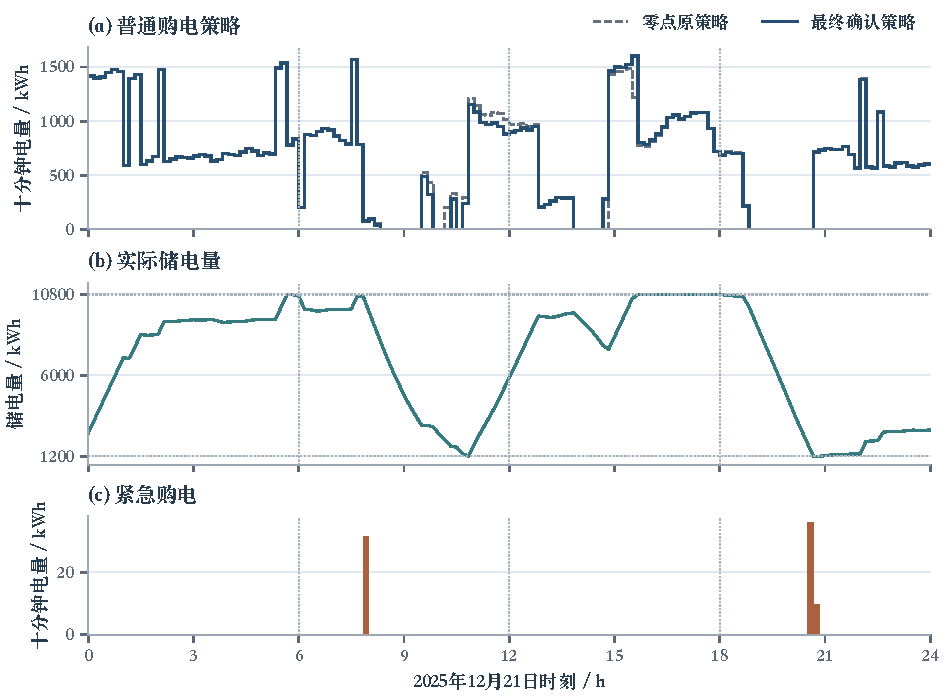
\includegraphics[width=\textwidth]{figures/q3/q3_dispatch.pdf}
    \caption{12月21日的普通购电量、实际储电量与紧急购电}
    \label{fig:q3-dispatch}
\end{figure}

\subsection{模型检验与日内预报价值}

独立复算覆盖48,096个区间，结果见表\ref{tab:q3-validation}。交易记录中的调整均位于对应六小时确认窗口，同一交付区间没有重复调整；决策只使用当时已经完成的历史数据。

\begin{table}[H]
    \centering\small
    \caption{问题三逐区间独立核验}
    \label{tab:q3-validation}
    \renewcommand{\arraystretch}{1.16}
    \begin{NiceTabularX}{\PaperTableNarrowWidth}{@{}lX[1]rX[2]r@{}}
\CodeBefore
  \rowcolor{paperpale}{1}
  \rowcolor{paperstripe}{3,5,7}
\Body
\toprule
核验对象 & & 最大绝对误差 & & 单位 \\
\midrule
母线供需平衡 & & $1.14\times10^{-12}$ & & kWh \\
累计储电量递推 & & $4.55\times10^{-11}$ & & kWh \\
跨区间状态连续 & & 0 & & kWh \\
储电量越界 & & 0 & & kWh \\
充放功率对应电量越界 & & $1.14\times10^{-13}$ & & kWh \\
总费用差 & & 0 & & 元 \\
\bottomrule
\end{NiceTabularX}
\end{table}

为判断日内预报的作用，在其他参数、初始储电量、策略窗口和DP设置相同的条件下，将6:00、12:00和18:00发布的光伏预报固定为零点版本，结果见表\ref{tab:q3-information}。

\begin{table}[H]
    \centering\small
    \caption{日内光伏预报更新的费用影响}
    \label{tab:q3-information}
    \renewcommand{\arraystretch}{1.16}
    \begin{tabularx}{\PaperTableCompactWidth}{@{}>{\columncolor{white}[0pt][\tabcolsep]}lRR>{\columncolor{white}[\tabcolsep][0pt]}R@{}}
\toprule
\rowcolor{paperpale} 光伏预报使用方式 & 总费用/万元 & 紧急电量/kWh & 年末储电量/kWh \\
\midrule
始终使用零点版本 & 1327.5193 & 48,425.57 & 2,448.95 \\
\rowcolor{paperstripe} 按0/6/12/18点更新 & 1320.7966 & 41,443.14 & 2,448.95 \\
\bottomrule
\end{tabularx}

\end{table}

两种方案年末储电量相同。使用日内更新后，总费用减少\QthreeInformationSaving{}元，紧急购电量由48,425.57\,kWh降至\QthreeEmergency{}\,kWh，因此保留6:00、12:00和18:00三个更新时刻。

\subsection{结论}

四个发布时间均按预先确定的协议使用，每次规划至日末并只确认随后六小时。2025年评估期总费用为\QthreeCostWan{}万元，日内预报更新在相同条件下节省\QthreeInformationRate\%。
